\chapter{Architettura a microservizi}
\label{cap:microservizi}

\begin{inbreve}
Il capitolo spiega come scomporre un sistema in servizi piccoli e indipendenti adatti al cloud. Parte dai servizi software
e dall'architettura orientata ai servizi, definisce i microservizi e ne mostra i motivi d'uso. Poi tratta le decisioni
di design: comunicazione, dati (con il teorema CAP e il pattern Saga), coordinamento, gestione dei guasti e
distribuzione. Chiude con vantaggi e svantaggi. Presuppone i capitoli~\ref{cap:architettura} (architettura)
e~\ref{cap:cloud} (cloud).
\end{inbreve}

\section{Servizi software}
\label{sec:micro-servizi}

Come si scompone un sistema in componenti? Tre esigenze guidano la risposta:
\begin{itemize}
  \item i componenti si possono sviluppare in parallelo da team diversi;
  \item si possono riusare, sostituire e distribuire su più computer;
  \item devono poter essere replicati facilmente, eseguiti in parallelo e migrati, per sfruttare scalabilità,
    affidabilità ed elasticità del cloud.
\end{itemize}
La conclusione è usare servizi \emph{stateless} che mantengono le informazioni persistenti in un database locale.

\begin{definizione}[Software service]
Un \termine{servizio software} è un componente accessibile via Internet.
\begin{itemize}
  \item Dato un input, produce l'output corrispondente, senza effetti collaterali.
  \item Si accede tramite la sua interfaccia pubblicata; i dettagli di implementazione sono nascosti.
  \item Non mantiene alcuno stato interno. Lo stato è conservato in un database o dal richiedente: può stare nella
    richiesta e il nuovo stato nel risultato.
  \item Può essere riallocato dinamicamente da un server virtuale a un altro, e questo dà scalabilità.
\end{itemize}
\end{definizione}

\subsection*{Dalla SOA ai microservizi}

\begin{itemize}
  \item \textbf{Service-oriented architecture} (SOA, fine anni '90): servizi indipendenti, autonomi, con interfacce
    pubbliche, implementati con tecnologie diverse.
  \item \textbf{Web Services} (inizio anni 2000): XML, SOAP, WSDL e decine di altri standard. Scambiavano dati XML grandi
    e complessi, con un overhead di gestione dei messaggi.
  \item \textbf{Sistemi orientati ai servizi moderni}: protocolli di interazione più semplici e leggeri, interfacce
    più semplici, formato più efficiente per i messaggi. Hanno overhead minore ed esecuzione più veloce.
\end{itemize}

Amazon ha ripensato che cosa debba essere un servizio:
\begin{itemize}
  \item un servizio deve riguardare una sola funzione di business;
  \item i servizi devono essere completamente indipendenti, ciascuno con il proprio database;
  \item un servizio gestisce la propria interfaccia utente;
  \item deve essere possibile sostituire o replicare un servizio senza cambiare gli altri.
\end{itemize}
Ne derivano i \termine{microservizi}: servizi stateless di piccole dimensioni con una singola responsabilità.

\section{Microservizi}
\label{sec:micro-microservizi}

I microservizi sono servizi piccoli che si possono combinare per costruire applicazioni. Sono indipendenti: l'interfaccia
di un servizio non è influenzata dai cambiamenti degli altri. Si può modificare e ridistribuire un servizio senza
cambiare né fermare gli altri.

\begin{table}[ht]
\centering
\small
\caption{Caratteristiche dei microservizi.}
\label{tab:micro-caratteristiche}
\begin{tabularx}{\linewidth}{>{\raggedright\arraybackslash}p{3.2cm}X}
\toprule
Caratteristica & Spiegazione \\
\midrule
Self-contained & Non hanno dipendenze esterne. Gestiscono i propri dati e implementano la propria interfaccia utente. \\
Lightweight & Comunicano con protocolli leggeri, quindi l'overhead di comunicazione è basso. \\
Implementation independent & Possono essere implementati con linguaggi di programmazione e tecnologie diversi (per
  esempio diversi tipi di database). \\
Independently deployable & Ogni microservizio gira in un processo proprio e si distribuisce in modo indipendente,
  con sistemi automatici. \\
Business-oriented & Implementano capacità ed esigenze di business, invece di offrire semplicemente un servizio tecnico. \\
\bottomrule
\end{tabularx}
\end{table}

\subsection{Coupling, cohesion e dimensione}

\begin{definizione}[Coupling e cohesion]
Il \termine{coupling} misura il numero di relazioni \emph{tra} componenti. Un coupling basso significa servizi
indipendenti e aggiornamenti indipendenti. La \termine{cohesion} misura il numero di relazioni \emph{dentro} un
componente. Una cohesion alta significa meno overhead di comunicazione tra servizi.
\end{definizione}

Vale il \termine{single responsibility principle}: ogni servizio deve fare una sola cosa e farla bene.

Quanto deve essere grande un microservizio? La regola è la ``\ingl{rule of twos}'':
\begin{itemize}
  \item un team può sviluppare, collaudare e distribuire il servizio in due settimane;
  \item il team si può sfamare con due pizze grandi (8--10 persone).
\end{itemize}

Un team così numeroso serve perché oltre alla funzionalità bisogna:
\begin{itemize}
  \item scrivere il codice che rende il servizio del tutto indipendente: elaborare i messaggi in arrivo e in uscita,
    gestire i guasti (del servizio e delle interazioni), gestire la coerenza dei dati usati da altri servizi, mantenere
    l'interfaccia del servizio;
  \item collaudare il servizio e le sue interazioni;
  \item supportare il servizio dopo la distribuzione.
\end{itemize}

\begin{esempio}[Servizi per l'autenticazione]
Un sistema usa un modulo di autenticazione che offre: registrazione utente, autenticazione con UID e password,
autenticazione a due fattori, gestione delle informazioni dell'utente, reset della password. Per identificare i
microservizi si procede così (\figrif{fig:micro-auth}):
\begin{itemize}
  \item si scompongono le feature a grana grossa in funzioni più dettagliate;
  \item si guardano i dati usati e si identifica un microservizio per ogni dato logico da gestire;
  \item si riduce al minimo la gestione di dati replicati.
\end{itemize}
\end{esempio}

\begin{figure}[ht]
\centering
\begin{tikzpicture}[blocco/.append style={minimum width=3.3cm, rounded corners=5pt},
  d/.style={draw, ellipse, minimum width=2.4cm, font=\small}]
\node[blocco] (a) at (0,0) {Authentication};
\node[blocco] (m1) at (4.2,1.3) {UID management};
\node[blocco] (m2) at (4.2,0) {Password management};
\node[blocco] (m3) at (4.2,-1.3) {User info management};
\node[d] (d1) at (8.8,1.3) {UID data};
\node[d] (d2) at (8.8,0) {Password data};
\node[d] (d3) at (8.8,-1.3) {User data};
\foreach \m in {m1,m2,m3} \draw (a.east) -- (\m.west);
\foreach \m/\d in {m1/d1,m2/d2,m3/d3} \draw[<->, thick] (\m) -- (\d);
\end{tikzpicture}
\caption{Microservizi del sistema di autenticazione. Ogni microservizio gestisce un solo dato logico e ha il proprio
database.}
\label{fig:micro-auth}
\end{figure}

\section{Perché usare i microservizi}
\label{sec:micro-motivi}

Due motivazioni:
\begin{enumerate}
  \item \textbf{Ridurre il lead time} per nuove feature e aggiornamenti, accelerando ricostruzione e ridistribuzione.
  \item \textbf{Scalare in modo efficace.} Ogni microservizio può essere distribuito in un container separato: si può
    fermare e riavviare rapidamente senza influire sugli altri e se ne possono distribuire rapidamente repliche.
\end{enumerate}

\textbf{Esempi.} Uber: nel 2014 un unico monolite Python, poi oltre 5\,000 microservizi. Spotify: 777 milioni di utenti attivi mensili (giugno 2026),
100 milioni di client concorrenti, 11--12 milioni di richieste al secondo al backend, circa 3\,000 servizi di
produzione. Utenti: Uber 208 milioni (giugno 2026), Netflix più di 325 milioni (dicembre 2025), Spotify 777 milioni
(giugno 2026).

\begin{esempio}[Sistema di stampa di foto per dispositivi mobili]
Un servizio permette agli utenti di caricare foto dal telefono, o indicare foto del loro account Instagram, da stampare
in formati e su supporti diversi (per esempio una tazza o una maglietta). Le stampe sono preparate e spedite a casa.
Si paga con un servizio come Android o Apple Pay, o registrando una carta di credito presso il fornitore del servizio.

Ci sono servizi separati per ogni area di funzionalità. Un \termine{API gateway} isola l'app dell'utente dai
microservizi del sistema, è un unico punto di contatto e traduce le richieste dell'app in chiamate ai microservizi
(\figrif{fig:micro-gateway}).
\end{esempio}

\begin{figure}[ht]
\centering
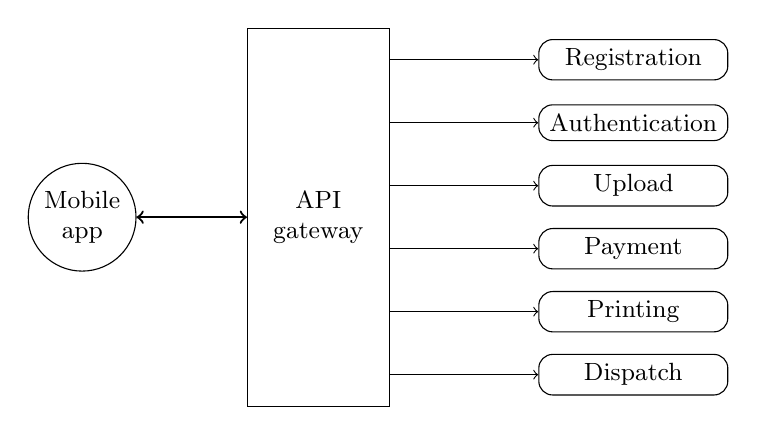
\begin{tikzpicture}[b/.style={draw, rounded corners=5pt, minimum width=2.4cm, font=\small}]
\node[draw, circle, font=\small, align=center, inner sep=2pt] (app) at (0,0) {Mobile\\app};
\node[draw, minimum width=1.8cm, minimum height=4.8cm, font=\small, align=center] (g) at (3,0) {API\\gateway};
\foreach \i/\n in {1/Registration, 2/Authentication, 3/Upload, 4/Payment, 5/Printing, 6/Dispatch} {
  \node[b] (s\i) at (7,{2.8-0.8*\i}) {\n};
  \draw[->] (g.east |- s\i.west) -- (s\i);
}
\draw[<->, thick] (app) -- (g);
\end{tikzpicture}
\caption{API gateway del sistema di stampa. L'app mobile parla solo con il gateway, che inoltra le richieste ai sei
microservizi.}
\label{fig:micro-gateway}
\end{figure}

\section{Decisioni di design}
\label{sec:micro-design}

I team di sviluppo di ogni servizio sono autonomi. Le decisioni architetturali riguardano cinque domande:
\begin{itemize}
  \item quali microservizi compongono il sistema?
  \item come devono comunicare tra loro (\rif{sec:micro-comunicazione})?
  \item come si distribuiscono e si condividono i dati (\rif{sec:micro-dati})?
  \item come si coordinano i microservizi (\rif{sec:micro-coordinamento})?
  \item come si rilevano, segnalano e gestiscono i guasti (\rif{sec:micro-guasti})?
\end{itemize}

Come scomporre il sistema in microservizi è \emph{difficile}:
\begin{itemize}
  \item non troppi: bassa cohesion, quindi overhead di comunicazione;
  \item non troppo pochi: alto coupling, quindi meno indipendenza negli aggiornamenti e nella distribuzione.
\end{itemize}

Alcuni consigli:
\begin{enumerate}
  \item bilanciare la funzionalità a grana fine e le prestazioni del sistema;
  \item seguire il \termine{common closure principle}: gli elementi che probabilmente cambiano insieme devono stare
    nello stesso servizio;
  \item associare i servizi alle capacità di business;
  \item i servizi devono accedere solo ai dati di cui hanno bisogno (più meccanismi di propagazione dei dati).
\end{enumerate}
Due punti di partenza: guardare per primi i dati che i servizi devono gestire; oppure partire da un monolite e
scomporlo più tardi.

\section{Comunicazione tra servizi}
\label{sec:micro-comunicazione}

\subsection{Sincrona e asincrona}

Nell'interazione \termine{sincrona} il servizio A chiama B e \emph{attende} la risposta. Nell'interazione
\termine{asincrona} A manda la richiesta e continua a elaborare. Le richieste passano per code (\figrif{fig:micro-sincrona}).

\begin{figure}[ht]
\centering
\begin{tikzpicture}[b/.style={draw, rounded corners=3pt, minimum width=1.9cm, minimum height=0.6cm, font=\footnotesize}]
\node[font=\small\bfseries\sffamily] at (2.4,0.8) {Sincrona};
\node[b] (a1) at (0,0) {Processing};
\node[b] (a2) at (2.7,0) {Waiting};
\node[b] (a3) at (5.4,0) {Processing};
\node[b] (b1) at (0,-1.8) {Processing};
\node[b] (b2) at (2.7,-1.8) {Processing};
\node[font=\footnotesize] at (-1.6,0) {Service A};
\node[font=\footnotesize] at (-1.6,-1.8) {Service B};
\draw[freccia] (a1) -- (a2); \draw[freccia] (a2) -- (a3);
\draw[freccia] (a1) -- node[right, font=\scriptsize] {calls} (b1);
\draw[freccia] (b1) -- (b2);
\draw[freccia] (b2) -- node[right, font=\scriptsize] {returns} (a2);
\begin{scope}[xshift=9.4cm]
\node[font=\small\bfseries\sffamily] at (1.6,0.8) {Asincrona};
\node[b] (c1) at (0,0) {Processing};
\node[b] (c2) at (3.2,0) {Processing};
\node[b] (q1) at (0,-1.1) {Queue B};
\node[b] (q2) at (3.2,-1.1) {Queue A};
\node[b] (d1) at (0,-2.2) {Processing};
\node[b] (d2) at (3.2,-2.2) {Processing};
\draw[freccia] (c1) -- (c2);
\draw[freccia] (c1) -- node[left, font=\scriptsize] {requests (B)} (q1);
\draw[freccia] (q1) -- (d1);
\draw[freccia] (d1) -- (d2);
\draw[freccia] (d2) -- node[right, font=\scriptsize] {requests (A)} (q2);
\draw[freccia] (q2) -- (c2);
\end{scope}
\end{tikzpicture}
\caption{Interazione sincrona (a sinistra): A chiama B, resta in attesa e riprende quando B restituisce il risultato.
Interazione asincrona (a destra): A e B non si attendono, perché si scambiano richieste attraverso code.}
\label{fig:micro-sincrona}
\end{figure}

\begin{itemize}
  \item[$+$] sincrona: più facile da scrivere e capire;
  \item[$+$] asincrona: coupling più debole, più efficiente;
  \item[$-$] asincrona: più difficile da scrivere e capire.
\end{itemize}

\subsection{Diretta e indiretta}

Nella comunicazione \termine{diretta} i messaggi sono inviati direttamente all'indirizzo del servizio. Nella
comunicazione \termine{indiretta} sono indirizzati al \emph{nome} del servizio e inviati a un \termine{message broker}.
Il broker trova l'indirizzo del servizio richiesto e può tradurre i messaggi. Un esempio di broker è RabbitMQ
(\figrif{fig:micro-broker}).

\begin{figure}[ht]
\centering
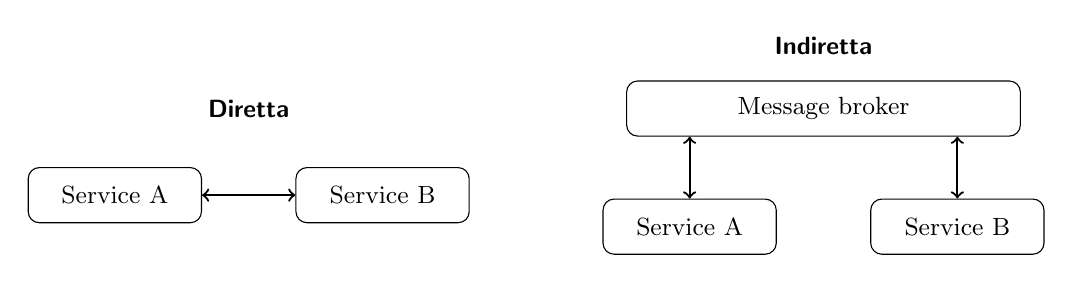
\begin{tikzpicture}[b/.style={draw, rounded corners=4pt, minimum width=2.2cm, minimum height=0.7cm, font=\small}]
\node[font=\small\bfseries\sffamily] at (1.7,1.1) {Diretta};
\node[b] (a) at (0,0) {Service A};
\node[b] (c) at (3.4,0) {Service B};
\draw[<->, thick] (a) -- (c);
\node[font=\small\bfseries\sffamily] at (9,1.9) {Indiretta};
\node[b, minimum width=5cm] (br) at (9,1.1) {Message broker};
\node[b] (a2) at (7.3,-0.4) {Service A};
\node[b] (c2) at (10.7,-0.4) {Service B};
\draw[<->, thick] (br.south -| a2) -- (a2);
\draw[<->, thick] (br.south -| c2) -- (c2);
\end{tikzpicture}
\caption{Comunicazione diretta tra due servizi e comunicazione indiretta attraverso un message broker.}
\label{fig:micro-broker}
\end{figure}

\begin{itemize}
  \item[$+$] diretta: più semplice e più veloce; $-$ chi richiede deve conoscere l'URI del destinatario;
  \item[$+$] indiretta: supporta interazioni sincrone e asincrone; è più facile modificare o sostituire i servizi;
    $-$ più complessa e più lenta.
\end{itemize}

\section{Distribuzione e condivisione dei dati}
\label{sec:micro-dati}

Ogni microservizio deve gestire \emph{i propri dati}. Per le dipendenze tra dati valgono tre regole:
\begin{enumerate}
  \item la condivisione dei dati deve essere la minima possibile;
  \item quasi tutta la condivisione deve essere in sola lettura, con pochi servizi responsabili degli aggiornamenti;
  \item serve un meccanismo che tenga coerenti le copie del database usate dai servizi replicati.
\end{enumerate}

\subsection{Coerenza dei dati}

Le architetture a database condiviso usano le transazioni \termine{ACID} per serializzare gli aggiornamenti ed evitare
incoerenze. In un sistema distribuito bisogna scegliere un compromesso tra coerenza dei dati e prestazioni. Quindi i
sistemi a microservizi vanno progettati per tollerare un certo grado di incoerenza. Se ne gestiscono due tipi:
\begin{itemize}
  \item \textbf{Dependent data inconsistency}: azioni o guasti di un servizio possono rendere incoerenti i dati gestiti da
    un altro servizio;
  \item \textbf{Replica inconsistency}: più repliche dello stesso servizio possono essere in esecuzione insieme, ciascuna con
    una propria copia del database e ciascuna che aggiorna la propria. Bisogna rendere questi database
    \termine{eventualmente coerenti} (\ingl{eventually consistent}).
\end{itemize}

\begin{esempio}[Coerenza eventuale\aggiunta]
Un servizio ha due repliche, A e B, ciascuna con il proprio database. Un utente cambia il suo indirizzo e la
richiesta arriva ad A. Per qualche istante A restituisce il nuovo indirizzo e B quello vecchio: le copie sono
\emph{incoerenti}. Dopo che A ha propagato l'aggiornamento a B, le due copie coincidono di nuovo. ``Eventualmente
coerente'' significa proprio questo: se non arrivano nuovi aggiornamenti, tutte le repliche prima o poi
convergono allo stesso valore. L'incoerenza è tollerabile quando un dato vecchio per pochi secondi non crea danni.
\end{esempio}

\subsection{Il teorema CAP}

\begin{teorema}[CAP, congettura di Brewer, 2000]
È impossibile che un servizio software fornisca contemporaneamente \emph{Consistency}, \emph{Availability} e
\emph{Partition-tolerance}, dove:
\begin{itemize}
  \item \textbf{Consistency} ($C$): ogni servizio restituisce la risposta ``giusta'' a ogni richiesta;
  \item \textbf{Availability} ($A$): ogni richiesta deve avere una risposta;
  \item \textbf{Partition-tolerance} ($P$): la rete può ritardare o perdere un numero arbitrario di messaggi tra i nodi.
\end{itemize}
\end{teorema}

In simboli il teorema dice $\neg(C \wedge A \wedge P)$. Nei sistemi distribuiti $P$ è vera, quindi:
\begin{align*}
\neg(C \wedge A \wedge P) &\equiv \neg(C \wedge A) && \text{($P$ è vera nei sistemi distribuiti)}\\
&\equiv \neg C \vee \neg A && \text{(leggi di De Morgan)}\\
&\equiv A \rightarrow \neg C && \text{(definizione di implicazione: $X \rightarrow Y \equiv \neg X \vee Y$)}\\
&\equiv C \rightarrow \neg A && \text{(definizione di implicazione)}
\end{align*}

Dunque se si garantisce la disponibilità ($A$) si rinuncia alla coerenza ($\neg C$) e viceversa. La
\figrif{fig:micro-cap} mostra perché $A \rightarrow \neg C$, con due server $S_1$ e $S_2$ che replicano il dato $d$ e due
client $C$ e $C'$. A sinistra tutti i messaggi arrivano e $C'$ legge il valore aggiornato. A destra l'aggiornamento
\texttt{update(d,v2)} verso $S_2$ si perde: $S_2$ \emph{risponde comunque} (è disponibile) ma restituisce il valore vecchio
$v_1$. Per rispondere ha rinunciato alla coerenza.

\begin{figure}[ht]
\centering
\begin{tikzpicture}[x=1cm, y=1cm, every node/.style={font=\scriptsize},
  msg/.style={->, >={Stealth[length=1.6mm]}}]
\newcommand{\vita}[2]{
  \foreach \x/\n in {0/C, 1.9/S1, 3.8/S2, 5.7/C'} {
    \node[font=\footnotesize] at (#1+\x,0) {\n};
    \draw[grigio] (#1+\x,-0.2) -- (#1+\x,#2);
  }}
% sinistra
\vita{0}{-5.1}
\draw[msg] (0,-0.7) -- node[above, sloped] {write(d,v1)} (1.9,-1.0);
\draw[msg] (1.9,-1.3) -- node[above, sloped] {ok} (0,-1.6);
\draw[msg] (1.9,-2.0) -- node[above, sloped] {update(d,v1)} (3.8,-2.3);
\draw[msg] (3.8,-2.6) -- node[above, sloped] {ok} (1.9,-2.9);
\draw[msg] (5.7,-3.5) -- node[above, sloped] {read(d)} (3.8,-3.8);
\draw[msg] (3.8,-4.1) -- node[above, sloped] {d=v1} (5.7,-4.4);
% destra
\begin{scope}[xshift=8.6cm]
\vita{0}{-8.1}
\draw[msg] (0,-0.7) -- node[above, sloped] {write(d,v1)} (1.9,-1.0);
\draw[msg] (1.9,-1.3) -- node[above, sloped] {ok} (0,-1.6);
\draw[msg] (1.9,-2.0) -- node[above, sloped] {update(d,v1)} (3.8,-2.3);
\draw[msg] (3.8,-2.6) -- node[above, sloped] {ok} (1.9,-2.9);
\draw[msg] (0,-3.5) -- node[above, sloped] {write(d,v2)} (1.9,-3.8);
\draw[msg] (1.9,-4.1) -- node[above, sloped] {ok} (0,-4.4);
\draw[msg, dashed, grigio] (1.9,-4.9) -- node[above, sloped] {update(d,v2)} (3.4,-5.1);
\node[rosso, font=\small\bfseries] at (3.6,-5.15) {$\times$};
\draw[msg] (5.7,-6.1) -- node[above, sloped] {read(d)} (3.8,-6.4);
\draw[msg, rosso] (3.8,-6.7) -- node[above, sloped] {d=v1} (5.7,-7.0);
\end{scope}
\node[font=\small\sffamily] at (2.85,-5.6) {Tutti i messaggi arrivano};
\node[font=\small\sffamily] at (11.45,-8.6) {L'aggiornamento v2 si perde};
\end{tikzpicture}
\caption{Perché $A \rightarrow \neg C$. A sinistra tutti i messaggi arrivano: $C'$ legge $d=v_1$, il valore corrente.
A destra l'aggiornamento \texttt{update(d,v2)} si perde (croce): $S_2$ risponde alla lettura con il valore vecchio
$d=v_1$ (in rosso), quindi è disponibile ma non coerente.}
\label{fig:micro-cap}
\end{figure}

\subsubsection{Conseguenze pratiche}
\begin{itemize}
  \item \textbf{Soluzione 1 ($A \wedge P$)}: garantire la disponibilità e offrire coerenza \emph{best-effort}. È la più usata
    nei microservizi, se la coerenza forte non è indispensabile. Si può fare un compromesso: per esempio tollerare dati
    vecchi di un'ora ma non di un giorno.
  \item \textbf{Soluzione 2 ($C \wedge P$)}: garantire la coerenza forte e offrire disponibilità \emph{best-effort}.
\end{itemize}

\subsection{Il pattern Saga}

Ogni transazione di business che coinvolge più servizi si implementa come \termine{saga}. Una saga è una sequenza di
\emph{transazioni locali}. Ognuna aggiorna un database e fa partire la transazione locale (o le transazioni) successiva
della saga. Se una transazione locale fallisce, la saga esegue una serie di \termine{transazioni compensative}.
La saga si coordina in due modi:
\begin{itemize}
  \item \textbf{Choreography}: ogni transazione locale pubblica un evento che fa partire la successiva;
  \item \textbf{Orchestration}: un \emph{orchestratore} dice ai partecipanti quali transazioni locali eseguire.
\end{itemize}
Le transazioni compensative seguono due modelli:
\begin{itemize}
  \item \textbf{Backward model}: annullano le modifiche fatte dalle transazioni locali già eseguite;
  \item \textbf{Forward model}: ``riprovare più tardi''.
\end{itemize}

\begin{esempio}[Una saga: prenotare un viaggio\aggiunta]
La prenotazione di un viaggio coinvolge tre servizi, ciascuno con il proprio database: noleggio auto, hotel, aereo.
La saga ha tre transazioni locali: $T_1$ prenota l'auto, $T_2$ prenota l'hotel, $T_3$ prenota il volo. Ogni
transazione locale ha la sua compensazione: $C_1$ cancella l'auto, $C_2$ cancella l'hotel.

Se tutto va bene, eseguire $T_1$, $T_2$, $T_3$ in sequenza conclude la saga. Se $T_3$ fallisce (nessun volo libero),
non esiste una transazione che annulli tutto insieme, perché i database sono separati. Nel \emph{backward model} si
eseguono le compensazioni in ordine inverso: $C_2$ poi $C_1$. Nel \emph{forward model} si riprova $T_3$ più tardi.
In \emph{choreography} ogni servizio, finita la propria transazione, pubblica un evento (``auto prenotata'') che
fa partire la successiva. In \emph{orchestration} un orchestratore chiama i tre servizi nell'ordine e, in caso di
fallimento, le compensazioni.
\end{esempio}

\subsection{L'approccio di Netflix}

Per replicare i dati in $n$ nodi: ``scrivere sui nodi che si riescono a raggiungere e sistemare dopo''. Si usa un
\termine{quorum}: per esempio devono rispondere $n/2 + 1$ repliche. L'approccio è quello associato ad Apache
Cassandra.

\begin{esempio}[Quorum con 5 repliche\aggiunta]
Con $n = 5$ servono $5/2 + 1 = 3$ risposte (la divisione è intera: $5/2 = 2$). Una scrittura riuscita su 3 repliche
è stata vista da una maggioranza. Una lettura che interroga 3 repliche incontra necessariamente almeno una replica
che ha ricevuto l'ultima scrittura, perché due maggioranze di 5 nodi hanno sempre un nodo in comune. Le 2 repliche
raggiunte in ritardo si ``sistemano dopo'', cioè si allineano in seguito. Il sistema continua a lavorare anche se 2
repliche sono irraggiungibili.
\end{esempio}

\section{Coordinamento dei servizi}
\label{sec:micro-coordinamento}

\begin{itemize}
  \item Nella \termine{service orchestration} un \emph{controllore esplicito} coordina i servizi.
  \item Nella \termine{service choreography} non c'è controllore: i servizi usano meccanismi publish\&subscribe
    (pubblicano e ricevono eventi).
\end{itemize}

\begin{figure}[ht]
\centering
\begin{tikzpicture}[b/.style={draw, rounded corners=4pt, minimum width=2.2cm, minimum height=0.8cm, font=\small, align=center}]
\node[font=\small\bfseries\sffamily] at (1.6,2.7) {Orchestration};
\node[b] (ct) at (1.6,1.7) {Authentication\\controller};
\node[b] (l1) at (0,0) {Login\\service};
\node[b] (p1) at (3.2,0) {Password\\service};
\draw (ct) -- (l1); \draw (ct) -- (p1); \draw[freccia] (l1) -- (p1);
\node[font=\small\bfseries\sffamily] at (9.2,2.7) {Choreography};
\node[b] (l2) at (7.6,1.7) {Login\\service};
\node[b] (p2) at (10.8,1.7) {Password\\service};
\node[draw, ellipse, minimum width=4.6cm, minimum height=0.8cm, font=\small] (ev) at (9.2,0) {Authentication events};
\draw[<->, dashed] (l2) -- (l2 |- ev.north);
\draw[<->, dashed] (p2) -- (p2 |- ev.north);
\end{tikzpicture}
\caption{Orchestrazione (a sinistra): un controllore decide quali servizi chiamare. Coreografia (a destra): i servizi
pubblicano e ricevono eventi, senza controllore.}
\label{fig:micro-coord}
\end{figure}

La choreography non ha un controllore esplicito ($+$), ma rende più difficili il debugging ($-$) e il recovery ($-$).
\textbf{Consiglio}: iniziare con l'orchestration e passare alla choreography solo se il prodotto è poco flessibile o
difficile da aggiornare.

\section{Gestione dei guasti}
\label{sec:micro-guasti}

Prima o poi qualcosa andrà storto, inevitabilmente: i servizi vanno progettati per far fronte ai guasti.

\begin{table}[ht]
\centering
\small
\caption{Tipi di guasto.}
\label{tab:micro-guasti}
\begin{tabularx}{\linewidth}{>{\raggedright\arraybackslash}p{3.8cm}X}
\toprule
Tipo di guasto & Spiegazione \\
\midrule
Internal service failure & Condizioni rilevate dal servizio e segnalate al richiedente con un messaggio di errore. Per
  esempio un servizio che riceve un URL in input e scopre che è un link non valido. \\
External service failure & Hanno una causa esterna che compromette la disponibilità di un servizio. Il servizio può
  smettere di rispondere e bisogna intervenire per riavviarlo. \\
Service performance failure & Le prestazioni del servizio calano a un livello inaccettabile. Può dipendere da un carico
  elevato o da un problema interno. Il monitoraggio esterno del servizio permette di rilevare i guasti di prestazione e
  i servizi che non rispondono. \\
\bottomrule
\end{tabularx}
\end{table}

\begin{esempio}[Disponibilità composta]
Un servizio offre la funzionalità $F$ chiamando altri due servizi, ognuno disponibile il 99\% del tempo e indipendenti
tra loro. $F$ è disponibile solo se lo sono entrambi: $0{,}99 \times 0{,}99 = 0{,}9801$. Quindi $F$ non è disponibile per
l'$1{,}99\%$ del tempo. In un giorno (86\,400 secondi) sono circa 1\,719 secondi, cioè circa 29 minuti. La risposta
più vicina tra 3 secondi, 30 secondi, 3 minuti e 30 minuti è \textbf{30 minuti}.
\end{esempio}

\subsection{Circuit breaker}

Il \termine{circuit breaker} funziona come un interruttore elettrico. Un client invoca un servizio remoto attraverso
un oggetto circuit breaker (\figrif{fig:micro-cb}).

\begin{figure}[ht]
\centering
\begin{tikzpicture}[b/.style={draw, rounded corners=4pt, minimum width=3.6cm, minimum height=1cm, font=\small, align=center}]
\node[b] (n) at (0,0) {Funzionamento normale:\\le chiamate passano};
\node[b] (t) at (9,0) {Interruttore scattato:\\per il tempo di timeout ogni\\chiamata fallisce subito};
\node[b] (x) at (4.5,-3.2) {Dopo il timeout: passano\\poche richieste di prova};
\draw[freccia] (n) -- node[above, font=\footnotesize, align=center] {guasti consecutivi\\oltre la soglia} (t);
\draw[freccia] ([xshift=-1.3cm]t.south) -- node[midway, fill=white, inner sep=1.5pt, font=\footnotesize, align=center] {timeout\\scaduto} (x.north east);
\draw[freccia] (x.west) -| (n.south);
\node[font=\footnotesize, anchor=east, align=right] at (-0.2,-1.8) {le richieste\\riescono};
\draw[freccia] (x.east) -| ([xshift=1.3cm]t.south);
\node[font=\footnotesize, anchor=west] at (6.7,-3.55) {falliscono: il timeout ricomincia};
\end{tikzpicture}
\caption{Circuit breaker. Quando i guasti consecutivi superano una soglia l'interruttore scatta e per un periodo di timeout
ogni chiamata fallisce subito. Scaduto il timeout passano poche richieste di prova: se riescono si riprende il
funzionamento normale, altrimenti il timeout ricomincia.}
\label{fig:micro-cb}
\end{figure}

\subsection{Tolleranza ai guasti e collaudo}

L'applicazione deve \emph{tollerare i guasti}. Per collaudarla in modo ``coraggioso'' si usa \termine{Chaos Monkey}:
uno strumento che termina a caso istanze di VM e container che girano nell'ambiente di produzione.

\section{Distribuzione dei servizi}
\label{sec:micro-distribuzione}

\subsection{DevOps}

Nell'approccio \termine{DevOps} lo stesso team è responsabile dello sviluppo (\emph{Dev}), della distribuzione e della
gestione (\emph{Ops}) del servizio.

\subsection{Continuous deployment}

La \termine{continuous deployment pipeline} (\figrif{fig:micro-pipeline}) parte quando si fa il commit di una modifica
al sistema di gestione delle versioni. Ogni controllo che fallisce fa rifiutare la modifica (\emph{reject change}).

\begin{figure}[ht]
\centering
\begin{tikzpicture}[b/.style={draw, rounded corners=4pt, minimum width=2.2cm, minimum height=0.9cm, font=\footnotesize, align=center}]
\node[font=\footnotesize, align=center] (c) at (0,2.0) {Commit change to\\version management};
\node[b] (u) at (0,0.5) {Run unit\\tests};
\node[b] (bt) at (3.4,0.5) {Build test\\system};
\node[b] (i) at (6.8,0.5) {Run integration\\tests};
\node[b] (co) at (6.8,-1.6) {Containerize\\service};
\node[b] (d) at (3.4,-1.6) {Deploy service\\container};
\node[b] (a) at (0,-1.6) {Run acceptance\\tests};
\node[b] (r) at (0,-3.4) {Replace current\\service};
\draw[freccia] (c) -- node[right, font=\scriptsize] {triggers} (u);
\draw[freccia] (u) -- node[above, font=\scriptsize] {pass} (bt);
\draw[freccia] (bt) -- node[above, font=\scriptsize] {pass} (i);
\draw[freccia] (i) -- node[right, font=\scriptsize] {pass} (co);
\draw[freccia] (co) -- (d);
\draw[freccia] (d) -- (a);
\draw[freccia] (a) -- node[right, font=\scriptsize] {pass} (r);
\node[font=\footnotesize, rosso, anchor=west, align=left] at (1.6,-3.4) {Se un test fallisce:\\reject change};
\end{tikzpicture}
\caption{Pipeline di continuous deployment. Dopo il commit: unit test, costruzione del sistema di test, integration test.
Se tutto passa, il servizio viene containerizzato, distribuito come container e sottoposto agli acceptance test. Solo
se anche questi passano sostituisce il servizio corrente. Un fallimento in qualsiasi passo fa rifiutare la modifica.}
\label{fig:micro-pipeline}
\end{figure}

\subsection{Monitoring e rollback}

Il collaudo non può prevenire il 100\% dei problemi imprevisti: bisogna \emph{monitorare} i servizi distribuiti. Se un
servizio ha un guasto, si può tornare alla versione precedente (\emph{rollback}).

\begin{esempio}[Rollback del servizio Cameras]
Quando si introduce una nuova versione di un servizio, si mantiene la vecchia e si cambia il ``\emph{current version
link}'' perché punti al nuovo servizio. Se il monitor rileva un problema con la nuova versione (``Cameras 002''), riporta
il link alla versione 001 del servizio Cameras (\figrif{fig:micro-rollback}).
\end{esempio}

\begin{figure}[ht]
\centering
\begin{tikzpicture}[b/.style={draw, rounded corners=4pt, minimum width=2.2cm, minimum height=0.8cm, font=\small, align=center}]
\node[draw, circle, font=\small, align=center, inner sep=1pt] (g) at (0,0) {API\\gateway};
\node[b] (c) at (3.2,0) {Cameras};
\node[b] (c2) at (8.6,1.0) {Cameras 002};
\node[b] (c1) at (8.6,-1.0) {Cameras 001};
\node[b] (m) at (5.8,2.8) {Service\\monitor};
\draw[freccia] (g) -- (c);
\draw[freccia, dashed] (c) -- node[above, font=\scriptsize, sloped] {current version link} (c2);
\draw[freccia, dashed, grigio] (c) -- (c1);
\draw[freccia] (c2.north) -- node[right, font=\scriptsize] {risposta} (m.south east);
\draw[freccia] (m.south west) -- node[left, font=\scriptsize] {segnala} (c.north);
\node[font=\footnotesize, align=right, anchor=east] at (-1.1,0) {richiesta\\del servizio};
\end{tikzpicture}
\caption{Rollback. Il servizio Cameras punta con il current version link alla versione 002. Il monitor controlla le
risposte: se rileva un problema, il link torna a 001, che è stata conservata.}
\label{fig:micro-rollback}
\end{figure}

\section{Considerazioni finali}
\label{sec:micro-conclusioni}

I \textbf{vantaggi} dei microservizi: tempi più brevi per nuove feature (\emph{lead time}) e scalabilità efficace.
Gli \textbf{svantaggi}:
\begin{itemize}
  \item overhead di comunicazione;
  \item complessità;
  \item i ``tagli sbagliati'' (scomposizioni mal fatte);
  \item evitare la duplicazione dei dati il più possibile, mantenendo i microservizi isolati, è una delle sfide maggiori;
  \item un team scadente produce sempre un sistema scadente.
\end{itemize}

\begin{attenzione}[Quando usare i microservizi]
M.~Fowler: non conviene nemmeno prendere in considerazione i microservizi se il sistema non è troppo complesso per essere
gestito come monolite. Per sistemi poco complessi il carico aggiuntivo di gestire i microservizi riduce la produttività.
\end{attenzione}

\begin{figure}[ht]
\centering
\begin{tikzpicture}
\draw[->, thick] (0,0) -- (8.4,0) node[below left, font=\footnotesize] {Base complexity};
\draw[->, thick] (0,0) -- (0,4.4) node[above, font=\footnotesize] {Productivity};
\draw[very thick, verde] plot[smooth] coordinates {(0.2,3.7) (2,3.6) (3.2,3.1) (4.1,1.4) (5,0.7) (6,0.55) (8,0.5)};
\draw[very thick, blu] plot[smooth] coordinates {(0.2,3.1) (2,3.0) (3.4,2.9) (4.6,2.2) (5.8,1.4) (6.6,1.3) (8,1.25)};
\node[verde, font=\footnotesize, anchor=west] at (8.1,0.5) {Monolith};
\node[blu, font=\footnotesize, anchor=west] at (8.1,1.25) {Microservice};
\end{tikzpicture}
\caption{Produttività in funzione della complessità di base del sistema (andamento qualitativo).
Per sistemi poco complessi il monolite è più produttivo. Oltre una certa complessità la produttività del monolite
cala rapidamente, mentre il minore coupling dei microservizi ne attenua il calo. Inoltre la competenza del team conta
più della scelta tra monolite e microservizi.}
\label{fig:micro-produttivita}
\end{figure}

\begin{puntichiave}
\begin{itemize}
  \item Un servizio è stateless, ha un'interfaccia pubblicata e può essere replicato e migrato. Un microservizio è piccolo,
    con una sola responsabilità, indipendente, con i propri dati.
  \item Coupling basso e cohesion alta; dimensione secondo la ``rule of twos'' (due settimane, 8--10 persone).
  \item Motivi: lead time più breve e scalabilità. L'API gateway isola l'app dai microservizi.
  \item Comunicazione: sincrona o asincrona, diretta o con message broker.
  \item CAP: non si possono avere insieme $C$, $A$ e $P$; con $P$ si sceglie tra $A$ (coerenza \emph{best-effort}) e $C$.
    Saga e quorum gestiscono la coerenza.
  \item Orchestration prima, choreography solo se necessario.
  \item Guasti: circuit breaker, applicazioni tolleranti, Chaos Monkey. Distribuzione: DevOps, continuous deployment,
    monitoring e rollback.
  \item Evitare i microservizi se il sistema non è troppo complesso per un monolite.
\end{itemize}
\end{puntichiave}

\begin{domande}
\begin{enumerate}
  \item Che cos'è un servizio software? Che cosa significa stateless?
  \item Quali caratteristiche ha un microservizio? Che cosa sono coupling e cohesion e che cos'è la rule of twos?
  \item Quali sono i motivi per adottare i microservizi? A che cosa serve l'API gateway?
  \item Quali consigli aiutano a scomporre un sistema in microservizi?
  \item Confrontare comunicazione sincrona e asincrona, diretta e indiretta.
  \item Enunciare il teorema CAP e dimostrare che $A \rightarrow \neg C$ quando $P$ è vera. Quali sono le due soluzioni pratiche?
  \item Che cos'è una saga? Come si coordina e come si compensano i fallimenti?
  \item Orchestration o choreography: differenze e consiglio.
  \item Se un servizio chiama due servizi indipendenti, ciascuno disponibile al 99\%, quanto è disponibile?
  \item Come funziona un circuit breaker? Che cos'è Chaos Monkey?
  \item Che cosa fa la continuous deployment pipeline? Come si fa il rollback?
  \item Quando non conviene usare i microservizi?
\end{enumerate}
\end{domande}
